\documentclass[a4paper,12pt]{article}
\usepackage[utf8]{inputenc}

%  Русский язык
\usepackage{multirow}
\usepackage{wrapfig}
\usepackage[T2A]{fontenc}			% кодировка
\usepackage[utf8]{inputenc}			% кодировка исходного текста
\usepackage[english,russian]{babel}	% локализация и переносы

\usepackage{indentfirst} %Красная строка
\usepackage[a4paper,top=1.3cm,bottom=2cm,left=1.5cm,right=1.5cm,marginparwidth=0.5cm]{geometry}
\usepackage[usenames]{color}
\usepackage{colortbl}
\usepackage{csvsimple}
\usepackage{siunitx}

\addto\captionsrussian{\def\refname{5   Список используемой литературы}}

% Заметки
\usepackage{todonotes}

% Математика
\usepackage{amsmath,amsfonts,amssymb,amsthm,mathtools} 
\usepackage{hyperref}

\renewcommand{\AA}{\ensuremath{\mathring{A}}}

\begin{document}
\def\figurename{Рисунок}
\begin{titlepage}
\begin{center}
    {\large МОСКОВСКИЙ ФИЗИКО-ТЕХНИЧЕСКИЙ ИНСТИТУТ (НАЦИОНАЛЬНЫЙ ИССЛЕДОВАТЕЛЬСКИЙ УНИВЕРСИТЕТ)}
\end{center}
\begin{center}
    {\largeФизтех-школа биологической и медицинской физики}
\end{center}

\vspace{1cm}
{\huge
\begin{center}
    {\bf Лабораторная работа по оптике}\\
    \vspace{0.5cm}
    4.5.2. Интерференция лазерного излучения.
\end{center}
}

\vspace{4cm}
\begin{flushright}
{\LARGE Выполнила студентка группы Б06-103:\\ Фитэль Алена \\}

\end{flushright}
\vspace{9cm}
\begin{center}
    Долгопрудный, 2023 г.
\end{center}
\end{titlepage}
\newpage


\section{Аннотация}

\textbf{Цель работы:} исследовать зависимость видности интерференционной картины от разности хода интерферирующих лучей и от их поляризации.

\textbf{В работе используются:} гелий-неоновый лазер, интерферометр Майкельсона с подвижным зеркалом, фотодиод с усилителем, осциллограф С1-76, поляроид, линейка.

\section{Теоретическая часть}

Лазер состоит из двух зеркал, составляющих лазерный резонатор, и расположенной между ними газообразной усиливающей среды, состоящей из гелия и неона. Характерное расстояние между зеркалами ~--~$0.2 \div 1 \m$. Излучение распространяется по резонатору в прямом и обратном направлениях. При этом максимальным усилением обладают волны, для которых набег фазы при полном обходе резонатора кратен $2 \pi$. Тогда можно сформулировать условие на разность частот излучения. Так как:
\[ \dfrac{2 \pi}{\lambda}2L = 2 \pi m,	\quad L=m\lambda, \quad \nu_{m}=\dfrac{mc}{2L}, \]
тогда:

\begin{equation}
\label{eq:cond}
\Delta \nu_{m}=\nu_{m+1}-\nu_{m}=\dfrac{c}{2L},
\end{equation}

где $L$ -- длина резонатора, $m$ -- целое число. Поэтому лазер генерирует отдельные типы колебаний, называемые модами, удовлетворяющие условию (\ref{eq:cond}). 

Спектральная ширина отдельной моды определяется добротностью резонатора лазера и мощностью излучения. В He-Ne лазере из-за малого усиления активной среды используются зеркала с высоким отражением. добротность резонатора большая и спектральная ширина моды может быть очень узкой, вплоть до единиц $\Hz$. Ввиду наличия тепловых флуктуаций длины резонатора типичная ширина моды составляет $10^5 \; \Hz$. Количество генерируемых мод определяется шириной спектра усиления активной среды. Эта ширина складывается из естественной ширины линии излучения атомов неона и доплеровского уширения, вызванного тепловым движением атомов. При температуре $400 \K$ ширина по полувысоте спектра излучения газообразного неона равна $1.5 \cdot 10^{9} \; \Hz$.

Вследствие тепловых флуктуаций длина резонатора меняется, в результате чего моды "переползают" с одного края контура на другой, там исчезают, а на другом краю рождаются новые. Таким образом температура нестабильность приводит к медленным изменениям амплитуд колебаний в лазерных модах и числа самих мод.

\begin{figure}[h!]
	\begin{center}
		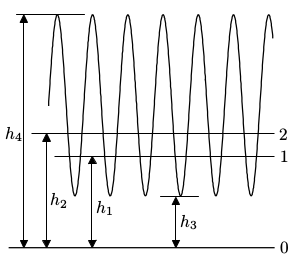
\includegraphics[scale = 0.5]{img1.png}
	\end{center}
	\caption{Осциллограмма сигналов фотодиода}
\end{figure}


\textbf{Видность интерференционной картины.} Если в плоскости наблюдения две плоские волны с длиной волны $\lambda_{0}$ сходятся под малым углом $\alpha$, то наблюдается интерференционная картина в виде последовательности темных и светлых полос c расстоянием между ними:
\begin{equation}
\label{eq:deltax}
\Delta x = \dfrac{\lambda_{0}}{\alpha}
\end{equation}

Для оценки чёткости интерференционной картины в окрестности некоторой точки используют параметр видимости:
\begin{equation}
\label{eq:seen}
V=\dfrac{I_{max}-I_{min}}{I_{max}+I_{min}},
\end{equation}

где $I_{max}$ и $I_{min}$ -- максимальная и минимальная интенсивности света интерференционной картины вблизи выбранной точки. Человеческий глаз может уверенно различать чередование светлых и темных полос при $V \geq 0,1$. 

Пусть интерферируют две волны с амплитудами $A_{m}$ и $B_{m}$. Если в точке наблюдения разность фаз между волнами равна $k_{m} l$, где $k_{m}$ -- волновое число, $l$ -- разность хода, то интенсивность света в этой точке:
\begin{equation}
\label{eq:intensity}
I_{m} = {A_{m}}^2+{B_{m}}^2+2 A_{m} B_{m} cos(k_{m}l)
\end{equation} 
В максимуме интенсивность $I_{max} = (A_{m}+B_{m})^2$, в минимуме $I_{min} = (A_{m}-B_{m})^2.$ Отсюда видность:
\begin{equation}
\label{eq:seen1}
V_{1} = \dfrac{2 \sqrt{\delta}}{1+\delta},
\end{equation}
где $\delta = (B_{m}/A_{m})^2$.

Рассмотрим влияние спекрального состава на видность интерференционной картины:
\begin{equation}
V_{2}(l) = \dfrac{\sum_{n=1}^{\infty} {A_{n}}^2 cos(\dfrac{2 \pi \Delta \nu n l}{c})}{\sum_{n=1}^{\infty}{A_{n}}^2}.
\end{equation}

Введем также поправку к видности, связанную с углом между плоскостями поляризации падающих волн:
\begin{equation}
V_{3} = cos \beta,
\end{equation}
где $\beta$ -- угол между плоскостями поляризации.
Кроме того, по данным осциллограммы (рис.1) можно определить
\begin{equation}
\delta = \dfrac{h_{1}}{h_{2}}
\end{equation}

\begin{equation}
V = \dfrac{h_{4}-h_{3}}{h_{4}+h_{3}},
\end{equation}

где $V$ -- полная видимость. Если имеют место все три фактора уменьшения видимости: неравенство амплитуд, несовпадение поляризаций и разная оптическая задержка между интерферирующими пучками, то:
\begin{equation}
V = V_{1} \cdot V_{2} \cdot V_{3}.
\end{equation}	
	
\section{Экспериментальная установка}


\begin{figure}[h!]
	\begin{center}
		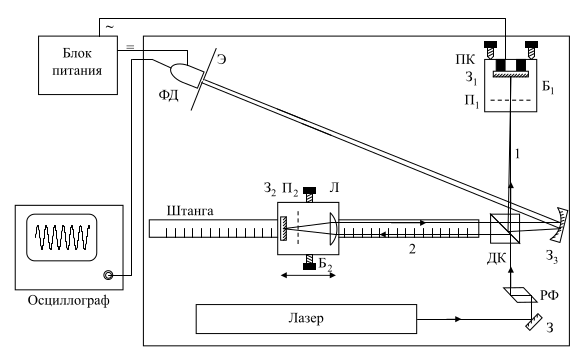
\includegraphics[scale = 0.5]{img2.png}
	\end{center}
	\caption{Схема экспериментальной установки}
\end{figure}


Экспериментальная установка представляет собой интерферометр Майкельсона, смонтированный на вертикально стоящей плите. Источником света служит гелий-неоновый лазер ($\lambda_{0} = 632,8 \nm$). Пучок лазерного излучения отражается от зеркала З и проходит через ромб Френеля(РФ).

Пучок 1 проходит поляроид $\text{П}_{1}$, отражается под небольшим углом от зеркала $\text{З}_1$, снова проходит поляроид $\text{П}_{1}$ и, частично отражаясь от диагональной плоскости делительного кубика, выходит из интерферометра, попадая на зеркало $\text{З}_3$ и фотодиод ФД. При этом можно вращать $\text{П}_{1}$, изменяя плоскость поляризации.

Пучок 2 проходит линзу Л, поляроид $\text{П}_2$, отражается от зеркала $\text{З}_2$, снова проходит $\text{П}_{2}$, линзу Л и делительный кубик, выходит из интерферометра, попадает на зеркало $\text{З}_3$ и далее на фотодиод ФД. Таким образом, от зеркала $\text{З}_3$ под небольшим углом друг к другу идут на фотодиод два пучка, проходящие через разные плечи интерферометра. Для питания усилителя сигнала фотодиода и управления пьезокерамикой используется блок питания БП.


\section{Обработка результатов}

\subsection{Влияние поляризации.}

Настроив поляроид на минимальную видимость и введя дополнительный поляроид, мы получаем интерференционную картину при его поворотах. Интенсивность излучения при вращении поляроида меняется, что говорит о его не хаотической поляризации. При вращении также изменяется интерференционная картина, что говорит о линейной или круговой поляризации.



\subsection{Зависимость видности от угла $\beta$ поворота поляроида.}



\begin{table}[h!]
\centering
\begin{tabular}{|c|c|c|c|c|c|c|c|c|c|}
\hline
$\beta$, град. & $\beta$, рад. & cos($\beta$) & h1, дел & h2, дел & h3, дел & h4, дел & V1   & V    & V3   \\ \hline
90       & 1,57    & 0,00   & 0,1     & 2,3     & 1,8     & 3,1     & 0,40 & 0,27 & 0,66 \\ \hline
80       & 1,40    & 0,17   & 0,2     & 2,3     & 1,6     & 3,2     & 0,54 & 0,33 & 0,61 \\ \hline
70       & 1,22    & 0,34   & 0,2     & 2,3     & 1,6     & 3,8     & 0,54 & 0,41 & 0,75 \\ \hline
60       & 1,05    & 0,50   & 0,3     & 2,4     & 1,2     & 4,2     & 0,63 & 0,56 & 0,88 \\ \hline
50       & 0,87    & 0,64   & 0,4     & 2,4     & 1,0     & 4,8     & 0,70 & 0,66 & 0,94 \\ \hline
40       & 0,70    & 0,77   & 0,6     & 2,4     & 0,8     & 5,2     & 0,80 & 0,73 & 0,92 \\ \hline
30       & 0,52    & 0,87   & 1,2     & 2,3     & 0,6     & 6,5     & 0,95 & 0,83 & 0,88 \\ \hline
20       & 0,35    & 0,94   & 1,5     & 2,2     & 0,8     & 7,0     & 0,98 & 0,79 & 0,81 \\ \hline
10       & 0,17    & 0,98   & 2,0     & 2,3     & 1,2     & 7,6     & 1,00 & 0,73 & 0,73 \\ \hline
0        & 0,00    & 1,00   & 2,1     & 2,3     & 1,6     & 7,4     & 1,00 & 0,65 & 0,65 \\ \hline
\end{tabular}
    \centering
    \label{table_v3}
        \caption{Измерения зависимости видности от угла}

\end{table}

\begin{figure}[h!]
	\begin{center}
		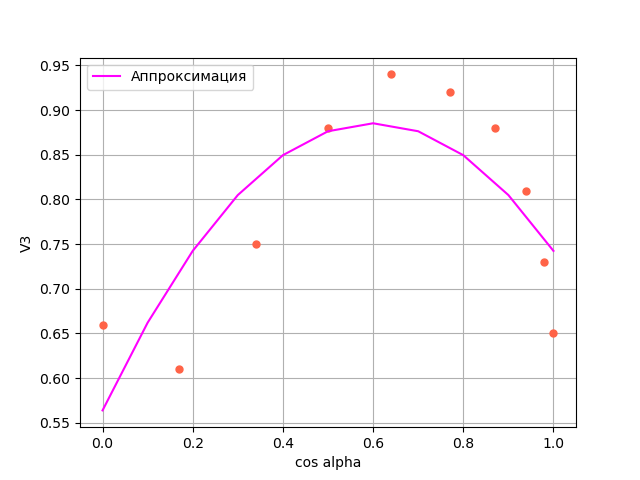
\includegraphics[scale = 0.8]{452_1.png}
	\end{center}
	\caption{График зависимости $ \nu({\cos}^2 \beta) $}
\end{figure}

\newpage
Исследуем зависимость видности интерференционной картины от угла
$ \beta $ поворота поляроида $ \text{П}_1 $ при нулевой разности хода ($ V_2 = 1 $). Для этого измерим величины $ h_1, h_2, h_3 \; \text{и} \; h_4 $ на экране осциллографа. Результаты занесем в таблицу (1) и построим график $V_3(\beta) = \dfrac{V}{V_1} = \dfrac{h_4 - h_3}{h_4 + h_3} \cdot \dfrac{h_2}{h_1}
$. Значения для $ \delta, V, V_1 $, получим из формул выше.
Полученная зависимость имеет вид $\cos(\beta)^2$. Таким образом, выполняется закон Малюса, следовательно полярирация наших волн линейная.

\subsection{Зависимость видности $\nu_2$ от координаты $x$ блока}

Теперь установим $ \beta $ на максимальную видность и будем перемещать блок $ \text{Б}_2 $, тем самым изменяя дальность хода $ x $. Аналогично предыдущему пункту измерим величины $ h_1, h_2, h_3 \; \text{и} \; h_4 $ на экране осциллографа. Результаты занесем в таблицу (2) и построим график $V_2 (x) = \dfrac{V}{V_1} = \dfrac{h_4 - h_3}{h_4 + h_3} \cdot \dfrac{h_2}{h_1}$. Значения для $ \delta, V, V_1 $ получим из формул выше, $V_3 = 1 (\beta = 0) $.





\begin{table}[h!]
\centering
\begin{tabular}{|c|c|c|c|c|c|c|c|c|}
\hline
$h_1$ & $h_2$ & $h_3$ & $h_4$ & L    & V     & $\delta$ & $V_1$ & $V_2$ \\ \hline
2,1   & 2,3   & 1,6   & 7,4   & 13   & 0,644 & 0,91     & 0,999 & 0,65  \\ \hline
1,9   & 1,6   & 1,4   & 5,6   & 16   & 0,600 & 1,19     & 0,996 & 0,60  \\ \hline
1,8   & 3,1   & 2,4   & 7,6   & 18   & 0,520 & 0,58     & 0,964 & 0,54  \\ \hline
1,8   & 2     & 2,5   & 5,4   & 20   & 0,367 & 0,90     & 0,999 & 0,37  \\ \hline
1,8   & 1,9   & 2,6   & 5     & 22   & 0,316 & 0,95     & 1,000 & 0,32  \\ \hline
1,8   & 0,9   & 2,2   & 3,4   & 24,5 & 0,214 & 2,00     & 0,943 & 0,23  \\ \hline
1,8   & 2     & 3,6   & 4,2   & 28   & 0,077 & 0,90     & 0,999 & 0,08  \\ \hline
1,8   & 2     & 3,2   & 4,1   & 31   & 0,123 & 0,90     & 0,999 & 0,12  \\ \hline
1,9   & 1,7   & 3,3   & 3,8   & 33   & 0,070 & 1,12     & 0,998 & 0,07  \\ \hline
1,9   & 2,8   & 4,2   & 5,4   & 36   & 0,125 & 0,68     & 0,981 & 0,13  \\ \hline
1,9   & 3,2   & 4,6   & 5,5   & 37   & 0,089 & 0,59     & 0,967 & 0,09  \\ \hline
1,9   & 2,8   & 4,2   & 5,05  & 35   & 0,092 & 0,68     & 0,981 & 0,09  \\ \hline
2     & 3,2   & 4,6   & 5,6   & 39   & 0,098 & 0,63     & 0,973 & 0,10  \\ \hline
2     & 3,2   & 4,6   & 5,8   & 42   & 0,115 & 0,63     & 0,973 & 0,12  \\ \hline
2     & 3     & 4     & 5,8   & 45   & 0,184 & 0,67     & 0,980 & 0,19  \\ \hline
2     & 3,8   & 5,4   & 6,2   & 48   & 0,069 & 0,53     & 0,951 & 0,07  \\ \hline
2     & 3,8   & 5,4   & 6,3   & 51   & 0,077 & 0,53     & 0,951 & 0,08  \\ \hline
2     & 3,6   & 5,2   & 6,1   & 54   & 0,080 & 0,56     & 0,958 & 0,08  \\ \hline
2     & 2     & 3,7   & 4,3   & 57   & 0,075 & 1,00     & 1,000 & 0,08  \\ \hline
2     & 4,8   & 6,5   & 7,2   & 59   & 0,051 & 0,42     & 0,911 & 0,06  \\ \hline
2     & 3,2   & 5     & 5,4   & 61   & 0,038 & 0,63     & 0,973 & 0,04  \\ \hline
2     & 2,1   & 3,8   & 4,6   & 64   & 0,095 & 0,95     & 1,000 & 0,10  \\ \hline
2     & 2,8   & 4     & 5,8   & 66   & 0,184 & 0,71     & 0,986 & 0,19  \\ \hline
2     & 4,1   & 5     & 6,2   & 67   & 0,107 & 0,49     & 0,939 & 0,11  \\ \hline
2     & 3     & 3,8   & 6     & 68   & 0,224 & 0,67     & 0,980 & 0,23  \\ \hline
2     & 3,1   & 3,1   & 7     & 70   & 0,386 & 0,65     & 0,976 & 0,40  \\ \hline
2     & 3,4   & 3     & 8     & 71,5 & 0,455 & 0,59     & 0,966 & 0,47  \\ \hline
2     & 2,8   & 2,3   & 74    & 73   & 0,940 & 0,71     & 0,986 & 0,95  \\ \hline
2     & 2,6   & 2     & 7,4   & 75   & 0,574 & 0,77     & 0,991 & 0,58  \\ \hline
2     & 2,4   & 1,8   & 7,3   & 77   & 0,604 & 0,83     & 0,996 & 0,61  \\ \hline
2     & 3,1   & 2     & 8,2   & 79   & 0,608 & 0,65     & 0,976 & 0,62  \\ \hline
2     & 2,1   & 1,8   & 6,6   & 81   & 0,571 & 0,95     & 1,000 & 0,57  \\ \hline
2     & 0,8   & 1,6   & 4,1   & 83   & 0,439 & 2,50     & 0,904 & 0,49  \\ \hline
2     & 0,4   & 1,8   & 3,2   & 86   & 0,280 & 5,00     & 0,745 & 0,38  \\ \hline
\end{tabular}
        \caption{Измерения зависимости видности от дальности хода}
    \label{table_v2}
\end{table}

\begin{figure}[h!]
	\begin{center}
		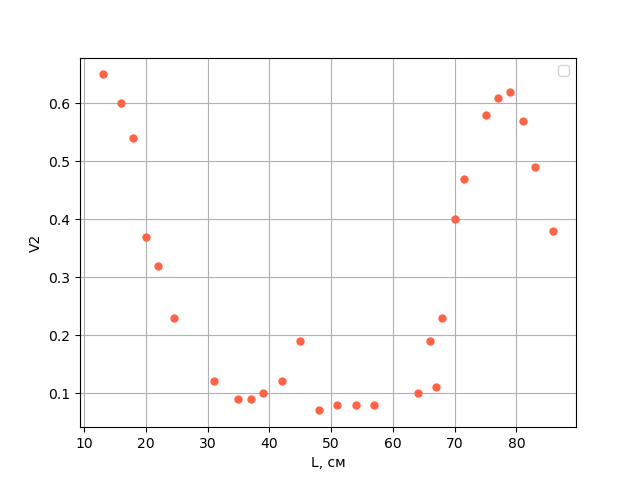
\includegraphics[scale = 0.8]{452_2.png}
	\end{center}
	\caption{График зависимости $ \nu_2(x)$}
\end{figure}



По полученному графику определим примерный размер резонатора лазера:
наблюдается 2 максимума по краям области измерения:$ x_1 \approx (10 \pm 1) \; \text{см} $ и $ x_2 \approx (79 \pm 1) \; \text{см} $:

\begin{equation}\label{}
L = \dfrac{1}{2} (x_2 - x_1) = (35.0 \pm 1.4) \; \text{см}
\end{equation}

Тогда межмодовое расстояние:
\[ \Delta \nu_m = \dfrac{c}{2L} =  (4,3 \pm 0,2) \cdot 10^8 \; \text{Гц} \]

Полуширина первого максимума: 
\[ l_{1/2} = (80 - 68) \text{ см} = (12.0 \pm 1.4) \text{ см} \]

Тогда диапазон частот, в котором происходит генерация продольных мод оценивается выражением:
\[\Delta F = \frac{0,6c}{ l_{1/2}} = (15 \pm 2)\cdot 10^8 \text{ Гц} \]

Оценим число генерируемых лазером продольных мод:
\[ n \approx 1 + 1.2\dfrac{L}{l_{1/2}} = 4.5 \pm 0.6\]
\newpage
\section{Вывод}
\begin{itemize}
    \item В первой части работы исследоалась поляризация волн, используемых в данной установке. Было установлено, что поляризация линейная или круговая.
    \item Была исследована зависимость видности интерференционной картины от угла поворота одного из поляроидов. Зависимость приближается функцией $ \cos^2 \alpha $, что означает, что поляризация излучения линейная.
    \item В ходе исследования зависимости видности от разности хода интерферирующих лучей в интерферометре Майкельсона,  было оценено расстояние $ L $ между зеркалами лазера, межмодовое расстояние:
    $L = (35.0 \pm 1.4) \text{ см}$, 
    $\Delta\nu_m = (4,3 \pm 0,2) \cdot 10^8 \text{ Гц}$.
    \item Была произведена  оцененка задержки $ l_{1/2} $. По этим данным был получен диапазон частот $ \Delta F $, в котором происходит генерация продольных мод, и приблизительное число мод:
    $ l_{1/2} = (12.0 \pm 1.4) \text{ см}$, 
    $\Delta F = (15 \pm 2)\cdot 10^8 \text{ Гц}$, 
    $n = 4.5 \pm 0.6$.
\end{itemize}

\end{document}
